\documentclass{article}
\usepackage[utf8]{inputenc}
\usepackage{graphicx}
\title{
\textbf{Research on Machine Learning and Its Algorithms and Development}
}
\author{
\textbf{Wei Jin}\\
Northwestern Polytechnical University Ming De College,Xi’an, Shaanxi, China
}
\begin{document}

\maketitle

\textbf{Abstract:}
 This article analyzes the basic classification of machine learning, including 
supervised learning, unsupervised learning, and reinforcement learning. It combines analysis 
on common algorithms in machine learning, such as decision tree algorithm, random forest 
algorithm, artificial neural network algorithm, SVM algorithm, Boosting and Bagging 
algorithm, BP algorithm. Through the development of theoretical systems, further 
improvement of autonomous learning capabilities, the integration of multiple digital 
technologies, and the promotion of personalized custom services, the purpose is to improve 
people's awareness of machine learning and accelerate the speed of popularization of machine 
learning.

\section{ Introduction}
With the rapid development of science and technology, artificial intelligence has also ushered in new 
development opportunities. Machine technology based on computer technology incorporates 
multidisciplinary theoretical knowledge, such as statistics and algorithm complexity, which further 
strengthens the functional attributes of artificial intelligence. By doing a reasonable analysis of 
machine learning algorithms, it can provide direction reference for subsequent machine learning 
development, thereby improving the applicability of machine learning algorithms and providing more 
convenience for the economic development of the industry

\section{Basic Classification of Machine Learning}

\subsection{\emph{Supervised Learning}}\\
In the process of machine learning, supervised learning belongs to a relatively basic learning method. 
This learning method refers to the establishment of corresponding learning goals by people before 
learning. During the initial training of the machine, the machine relies on information technology to 
learn the needs of learning. In order to collect basic data information, we are supposed to gradually 
complete the required learning content in a supervised environment. Compared with other learning 
methods, supervised learning can fully stimulate the generalized learning potential of the machine 
itself. After completing the system learning, it can help people to solve some classification or 
regression problems, which is highly systematic. Currently, the classic learning methods commonly 
used include BN, SVN, KNN, etc. Because the entire learning process has purpose, the machine 
learning process presents a certain regularity, and the learning content is more systematic [1].
\\\\
\subsection{\emph{Unsupervised Learning}}\\
Corresponding to supervised learning is unsupervised learning. The so-called unsupervised learning 
means that the machine does not mark the content in a certain direction during the entire learning process, but rely on the machine itself to complete the analysis of data information. In practice, the 
operation method is to let the machine learn the basic concepts and content, and then give the machine 
enough freedom to complete a series of content learning, including concepts and content similar to the 
basic principles, such as tree roots. In general, the continuous improvement of learning in stages has 
increased the breadth of machine learning content. At present, unsupervised learning includes 
algorithms such as deep belief networks and autoencoders. Such situations are conducive to the 
solution of clustering problems and have good applications in the development of many industries [2].
 \\\\
\subsection{\emph{Reinforcement Learning}}\\
In addition to supervised learning and unsupervised learning, there are also application methods of 
reinforcement learning in machine learning. The so-called reinforcement learning is the systematic 
learning of a certain content. In the specific application process, the data collected in the previous 
period will be used. It organizes and processes the feedback information of a certain part to form a 
closed loop of data processing. On the whole, reinforcement learning is a type of learning method that 
expands data collection based on statistics and dynamic learning. Such methods are mainly used to 
solve the control problem of robots. Its representative learning methods include Q-learning algorithm 
and Temporal difference learning algorithm.

\section{Analysis of Commonly Used Algorithms for Machine Learning
}
\subsection{\emph{Decision Tree Algorithm}}\\
Among the commonly used algorithms for machine learning, the decision tree algorithm belongs to 
the classic algorithm content. Its working principle is that when processing data information, it starts 
from the root node of the collection instance and reaches the position where the nodes meet to make it 
complete. Scientific division of practical examples. In order to facilitate the analysis of data 
information, the decision number algorithm will continue to split branches, and at the same time, the 
branches will be trimmed to improve the integrity of the data content [3]. From the point of view of 
calculation, the algorithm belongs to the top-down algorithm. During the content analysis process, the 
content of the node is analyzed for the optimal attributes, and then the node is expanded to more than 
two based on the node. This way, you can get comprehensive data information of the split, and the 
branching method like a tree can also increase the number of samples that can be analyzed, and at the 
same time determine the content that contains the most samples in the classification according to the 
sample number statistics. For example, when analyzing data, you can name the decision tree with a 
large amount of data information as the larger tree A, and set the upper limit of branch splitting. If the 
upper limit is set to 5, the larger tree A is in the classification after reaching the value of 5, it will 
stop continuing to split, and at the same time use the pruning strategy to process the larger tree model, 
so as to refine the data and improve the scientificity of the data analysis results.
\\\\

\subsection{\emph{Random Forest Algorithm}}\\
Similar to the decision tree algorithm, in the process of data calculation, the random forest algorithm 
can be used for further processing. The random forest algorithm will play a good role in controlling 
unreasonable data in the process of actual use. Thereby effectively improving the scientificity of the 
data split results and the accuracy of the data analysis results. At the same time, in the process of data 
analysis, multiple sets of classification trees will be created at the same time, and then the unified 
algorithm will be used for regression processing. Assuming the decision tree is an independent set ai (i 
= 1,2,3 ... n), then the random forest is the total set A, where A = {a1, a2, a3, ..., an}, where a = 1,2,3 ... 
n. Each set remains independent, and the distribution is a state of random distribution. When 
evaluating the classification data information, it will be selected by means of voting. The classification 
with the highest number of votes in the voting will output the vector value xi, and then the vector 
content will be classified to calculate the average value of different score states and provide data 
reference for the final judgment [4].
\\\\
\subsection{\emph{ Artificial Neural Network Algorithm}}\\
The so-called artificial neural network refers to imitating the process of human information 
transmission, classifying different data into one neuron, and connecting the data neurons with the help 
of the Internet to achieve complex memory activities. However, the artificial neural network algorithm 
is based on this unfolding data analysis process. Among the delineated neurons, each digital unit has a 
high degree of authenticity, and the data can complete the process of external output. It's just like the 
human body moves forward, stops, and runs. In the artificial neural network algorithm, the data 
information presented has a variety of application characteristics, and the corresponding analysis 
process can be completed according to actual needs. At present, commonly used artificial neural 
networks include multilayer forward neural networks MLFN, self-organizing neural networks, SOM, 
and ART [5]. In order to facilitate the analysis and calculation of the data, we can set the weighting 
coefficient in advance and then set the output threshold. After the calculated sum exceeds this value, a 
certain value is output to the outside, thereby improving the orderliness of the entire numerical 
analysis process.
\\\\

\subsection{\emph{SVM Algorithm}}\\
In the process of machine learning, the SVM algorithm also belongs to the commonly used algorithm 
content. In the specific application process, the algorithm mainly relies on the vector machine method 
to complete the established data analysis work. At the same time, the SVM algorithm will use the 
automatic support of the SVM to analyze the data information to be processed, so as to optimize the 
data information. In order to improve the scientificity of the final data analysis results, in the actual 
analysis process, multiple sets of analysis samples need to be collected to determine the sample data of 
the boundary value. For example, assuming that the data information to be processed is H (d), when 
processing it, first, the data information is processed centrally with the help of SVM technology so that 
it can be completely dispersed. Secondly, the boundary of the H (d) plane is determined from the 
maximum distance of the entire plane. Finally, the vector content of the H (d) plane is analyzed to 
obtain the output vector, which improves the accuracy of data processing.
\\\\
\subsection{\emph{Boosting and Bagging Algorithm}}\\
Boosting algorithm as a new type of machine algorithm content, its biggest application advantage is 
that it can complete the accurate processing of data information and improve the accuracy of the final 
processing result. In practice, the function prediction system will be built with the help of Boosting 
algorithm, and the system content will be continuously optimized with the help of reinforcement 
learning mode, thereby speeding up the processing of data information. AdaBoost is a relatively basic 
application in the Boosting algorithm. At the same time, AdaBoost is also an important guarantee for 
the expansion of the Boosting algorithm. The Bagging algorithm has a high similarity in the data 
processing process. In actual application, the difference is that the Bagging algorithm randomly selects 
the training set. And during the calculation of the function model, the Bagging algorithm does not 
analyze the weight content, and we need to continuously optimize the data model with the help of 
training to improve the accuracy of the data analysis results.
\\\\

\subsection{\emph{BP Algorithm}}\\
The BP algorithm belongs to supervised learning. The basic principle of the algorithm is shown in 
Figure 1.The figure shows a shallow forward neural network computing model, which includes an 
input layer, a hidden layer, and an output layer. A large number of neurons are connected to each other 
as network nodes. Each neuron processes the connection strength signals as network weights through 
an excitation function. By adjusting these connection strengths, the pattern information contained in 
the input data is mapped to the output layer.\\\\
\begin{figure}
    \centering
    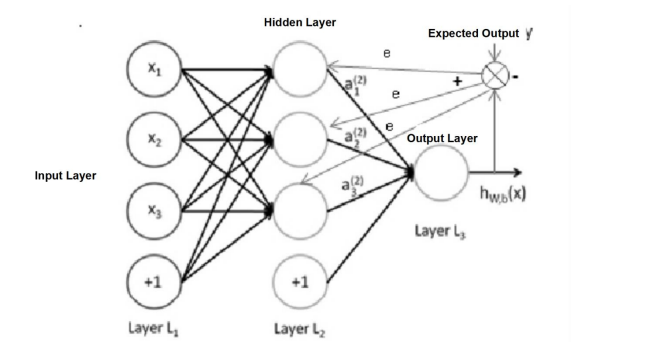
\includegraphics[width=1.0\linewidth]{figure.png}
    \caption{ Basic Principles of Algorithm Applicatio}
    \label{fig:my_label}
\end{figure}

As can be seen from the above figure, the direction of the information flow of forward propagation 
is input layer → hidden layer → output layer, and its mathematical model is:\\ 
h_w_.b^(X) =f(\sum^n_i_=_1      W_iX_i+b)
.

Where Wi and b are their weights and bias parameters, f (W, b; x): R 
→ R is called the excitation function, and sig-moid can be selected in practical applications , Tanh, 
ReLU and other functions or their variants, hW,b(x) are the network output values. In practical 
applications, the BP algorithm can be implemented by the steepest descent method, Newton method 
and its improved algorithm, quasi-Newton method and its correction algorithm, etc. At present, the 
L-BFGS algorithm is most widely used, and non-precise line search methods are often used to 
complete the optimization. This method follows Wolfe's criterion and Armijo's criterion, which 
guarantees the balance between the decline of the cost function and the convergence of the iterative 
sequence.\\\\
\section{Classic AI Technic for Deep Rainforcement}

Machine learning techniques are divided in two types: supervised learning, which trains a model that takes known data set (a labeled training set) as input and generates a model that can predict future output of new data. Unsupervised learning takes a dataset (unlabeled) and find patterns or intrinsic structures in data, it usually works as clustering data. Some of the most important techniques of machine learning are classify in table 1.\\

\begin{tabular}{|c|c|c|}

\hline
\textbf{Classification} & \textbf{Regression} & \textbf{Clustering} \\
\hline
Support Vector Machines & Linear Regression & K-Means \\
\hline
Discriminant Analysis & SVR & Fussy C-Means \\
\hline
Naive Bayes & Decision Trees & Hidden Markov Model \\
\hline
Nearest Neighbour & Neural Networks & Hebbian Learning \\
\hline
\end{tabular}

\section{Research on Machine Learning Development}
\subsection{\emph{Theoretical System Continues to Mature}}

In the future development process, the mechanical theory system will also be further optimized, and its 
content branches and coverage will also be expanded. In the initial formulation process of machine 
learning content, its content is mainly applicable to some automation industries, and the content of the 
entire theoretical system has not been completely sound. In practical application, the content of its 
theoretical system is not applicable in some fields. In response to such situations, the next stage of 
machine learning theory will be continuously strengthened, and the degree of refinement of the content 
will also be strengthened, which provides convenient conditions for the subsequent promotion of 
machine learning.
\\\\

\subsection{\emph{Autonomous Learning Ability is Further Improved}}
At present, many enterprises in China have realized the development model of automation, and 
intelligence is the focus of the next stage of development. In the context of the rapid development of Internet technology, the autonomous learning ability of machines will be further strengthened. 
Whether it is supervised learning or unsupervised learning, the autonomy that machine learning can 
master will continue to increase. In the future learning process of the machine, the machine will 
perform targeted or extensive learning according to its own needs, which also reduces the economic 
cost of the enterprise to update the equipment structure, thereby laying a solid foundation for the stable 
development of the enterprise economy.
\\\\
\subsection{\emph{Integration of Multiple Digital Technologies}}
At this stage, relying on Internet technology has produced many branch technologies, such as Internet 
of Things technology, digital technology, cloud computing technology, etc. These technologies can 
provide many convenient conditions in the process of data calculation. Although these digital 
technologies are still in the initial stage of integration, with the rapid development of technology, the 
integration of digital technology is also constantly improving. Besides, in the future development 
process, these technologies will be combined with algorithms to form a new technology application 
system, thereby laying a foundation for the further improvement of data analysis speed.
\\\\
\subsection{\emph{Promotion of Personalized Customization Services}}
With the continuous improvement of socio-economic level, people's requirements for personalized 
applications are also constantly rising, which is also one of the important development directions of 
machine learning in the future. With the continuous improvement of the intelligent level of mechanical 
learning, different application modules can be set up according to the actual needs of users. After 
obtaining the user request message, the data module can filter out the corresponding information 
content and match the corresponding service content at the same time to meet the user's personalized 
needs and improve user service satisfaction.

\section{Conclusion}
In summary, machine learning is still in its infancy, and it mainly relies on supervised learning, and 
does not fully overcome weak artificial intelligence. Relevant personnel need to constantly improve 
the theoretical foundation and practice of machine learning. In the corresponding scientific field and 
the development of computer technology, we should provide a good environment for machine learning, 
and the development prospect of machine learning is very broad. In addition, it is also necessary to 
actively learn from the experiences and lessons of developed countries, set up machine algorithms 
suitable for the development of domestic enterprises, and provide technical support for the economic 
development of the industry.
\\\\

\textbf{References}

[1] Li Kanghua, Jiang Shan. Machine Learning and Cultural Production Reform——Based on the 
       Perspective of the Development of AI Technology [J]. Journal of Xiangtan University 
       (Philosophy and Social Sciences), 2020, 44 (01): 74-79.
\\

 [2] Jiang Na, Yang Haiyan, Gu Qingchuan, Huang Jiya. Machine learning and its algorithm and 
      development analysis [J]. Information and Computer Science (Theoretical Edition), 2019
      (01): 83-84 + 87.
\\ 

   [3] Li Zhiwei. Development of machine learning and several learning methods [J]. Industry and 
     Science Forum, 2018, 15 (10): 198-199.
     \\ 
     
     [4] Zhang Run, Wang Yongbin. Research on machine learning and its algorithm and development [J]. 
    Journal of Communication University of China (Natural Science Edition), 2018, 23 (02): 
      10-18 + 24.
      \\
      
    [5] Zhang Changshui. Research on the development of machine learning and data mining [C].. 
    2010-2011 Development Report of Control Science and Engineering Discipline.: Chinese 
    Society of Automation, 2018: 82-89 + 223

\end{document}
